\documentclass[10pt,aspectratio=169,dvipsnames]{beamer}
\usetheme[]{Berlin}

\setbeamertemplate{footline}{
  \usebeamercolor[fg]{framesource}%
  \usebeamerfont{page number in head}%
  \hspace{0.2cm}
  \small \insertframenumber
  \vspace{0.2cm}
  \doclicenseIcon
  \hfill
  
\includegraphics[height=0.8cm]{graphics/logos/tub_logo.pdf}
  \hspace{0.2cm}
}

\setbeamercovered{transparent}

% wider right margin so content doesn't run into the footer logo
\setbeamersize{text margin left=1cm, text margin right=1.8cm}

\setbeamertemplate{footline}[
 myframe number]

% PACKAGES
\usepackage[absolute,overlay]{textpos}
\usepackage[utf8]{inputenc}
\usepackage[official]{eurosym}
\usepackage{booktabs,multicol,multirow,tabularx,array}
\usepackage{subcaption}
\usepackage{parskip}
\usepackage{bm}
\usepackage{tikz}
\usepackage{adjustbox}
\usepackage[super]{nth}
\usepackage[version=4]{mhchem}
\usepackage{siunitx}
\usepackage{tikz}
\usetikzlibrary{calc}


\sisetup{
  detect-all = true
}


\usepackage[
    type={CC},
    modifier={by},
    version={4.0},
]{doclicense}

% HYPERREFERENCES
\usepackage{hyperref}
\hypersetup{
	colorlinks=true,
	citecolor=tub-blue,
	linkcolor=tub-blue,
	urlcolor=tub-blue
}

\usepackage[sfdefault]{roboto}
\usepackage[normalem]{ulem}

% \usepackage[backend=biber,style=numeric-comp]{biblatex}
% \addbibresource{references.bib}

\newcolumntype{R}[1]{>{\raggedleft\arraybackslash}p{#1}}


% GRAPHICS
\graphicspath{
    {graphics/},
  }
\DeclareGraphicsExtensions{.pdf,.jpeg,.png,.jpg}

% FORMATTING
\setlength{\parskip}{6pt}
\linespread{1.1}
\newcommand{\seprule}{\par\noindent\textcolor{black!25}{\rule{\textwidth}{0.4pt}}}

% SOURCES
\setbeamercolor{framesource}{fg=gray}
\setbeamerfont{framesource}{size=\tiny}
\newcommand{\source}[1]{\begin{textblock*}{10cm}(3.6cm,8.25cm)
    \begin{beamercolorbox}[ht=0.5cm,right]{framesource}
        \usebeamerfont{framesource}\usebeamercolor[fg]{framesource} Source: {#1}
    \end{beamercolorbox}
\end{textblock*}}

% REFERENCES
% \usepackage[style=nature, doi=true, maxcitenames=3]{biblatex}
% \bibliography{bibliography}
% \renewcommand*{\bibfont}{\footnotesize}

% COLOR TEXT
\newcommand{\bl}[1]{\textcolor{tub-blue}{#1}}
\newcommand{\gr}[1]{\textcolor{tub-green}{#1}}
\newcommand{\rd}[1]{\textcolor{tub-red}{#1}}
\newcommand{\yl}[1]{\textcolor{tub-yellow}{#1}}
% \newcommand{\org}[1]{\textcolor{tub-orange}{#1}}
\newcommand{\cb}[1]{\colorbox{gray!20}{#1}}

\usepackage{array}% https://ctan.org/pkg/array
\makeatletter
\g@addto@macro{\endtabular}{\rowfont{}}% Clear row font
\makeatother
\newcommand{\rowfonttype}{}% Current row font
\newcommand{\rowfont}[1]{% Set current row font
   \gdef\rowfonttype{#1}#1%
}
\newcolumntype{L}{>{\rowfonttype}l}

\usepackage[most]{tcolorbox}
\tcbuselibrary{listingsutf8}

% Custom commands
\usepackage{caption}
\renewcommand{\figurename}{} % Removes the "Figure" text
\captionsetup[figure]{labelformat=empty, labelsep=none} % Removes numbering and colon


% FONT
%\usepackage{utopia}

% REFERENCES
%\usepackage[backend=biber,style=authoryear-comp]{biblatex}
%\bibliography{references.bib}

% DECK-SPECIFIC
\usepackage{fontawesome5}
\colorlet{ink}{black}
\colorlet{mute}{black!60}
\colorlet{rule}{black!25}
\colorlet{inv}{tub-blue}
\colorlet{adv}{tub-red}
\colorlet{rec}{tub-green}
\colorlet{panel}{tub-blue!8}

% take-away line under a figure
\newcommand{\takeaway}[1]{%
  \par\smallskip
  \colorbox{panel}{\parbox{\dimexpr\linewidth-2\fboxsep}{\footnotesize\strut#1\strut}}}

% placeholder box: \placeholder{width}{height}{text}
\newcommand{\placeholder}[3]{%
  \tikz{\node[draw=mute,dashed,thick,fill=panel,rounded corners=2pt,minimum width=#1,
    minimum height=#2,text width=\dimexpr#1-0.4cm\relax,align=center,font=\scriptsize\color{mute}]
    {\faImage\ \textbf{Placeholder}\\[0.2em]#3};}}

% "ONGOING WORK" label along the right edge, for single frames
\newcommand{\ongoing}{%
  \begin{textblock*}{0.5cm}(\paperwidth-0.5cm,0cm)
    \rotatebox{90}{\makebox[\paperheight][c]{\color{black!25}\fontsize{8}{8}\selectfont\bfseries ONGOING WORK}}
  \end{textblock*}}

% Two slides for the RESILIENT final workshop, 20 November 2026, Fraunhofer ENIQ, Berlin
% (https://resilient-project.github.io/final-workshop/), to be merged into the project summary talk.
% No title slide on purpose.

\begin{document}

% SLIDE 1: OPEN GRID DATA (follows the OSM slide of 20251106_dena_exchange.tex)
\begin{frame}{Electricity high-voltage grid based on OpenStreetMap (OSM)}
	\begin{columns}
		\begin{column}{0.64\textwidth}
			\footnotesize
			\begin{itemize}
				\setlength\itemsep{.8em}
				\item Dataset contains a topologically connected representation of the \alert{European high-voltage grid} (220\,kV to 750\,kV), constructed using \alert{OpenStreetMap} data
				\item ${\sim}$5\,800 buses, ${\sim}$7\,300 AC lines and all European HVDC connections, validated against ENTSO-E statistics; released under an \alert{open licence} (ODbL)
				\item \alert{Default transmission grid in PyPSA-Eur} since 2024, regularly updated as OSM data improves
				\item \alert{grid-builder}: standalone, modular workflow to build the grid for any country from the latest OSM data, incl.\ an interactive map linking every element to its source
				\item Transparent, reproducible grid data that anyone can check, correct and reuse, e.g.\ to draw the outage islands in RESILIENT (next slide)
			\end{itemize}
		\end{column}
		\begin{column}{0.36\textwidth}
			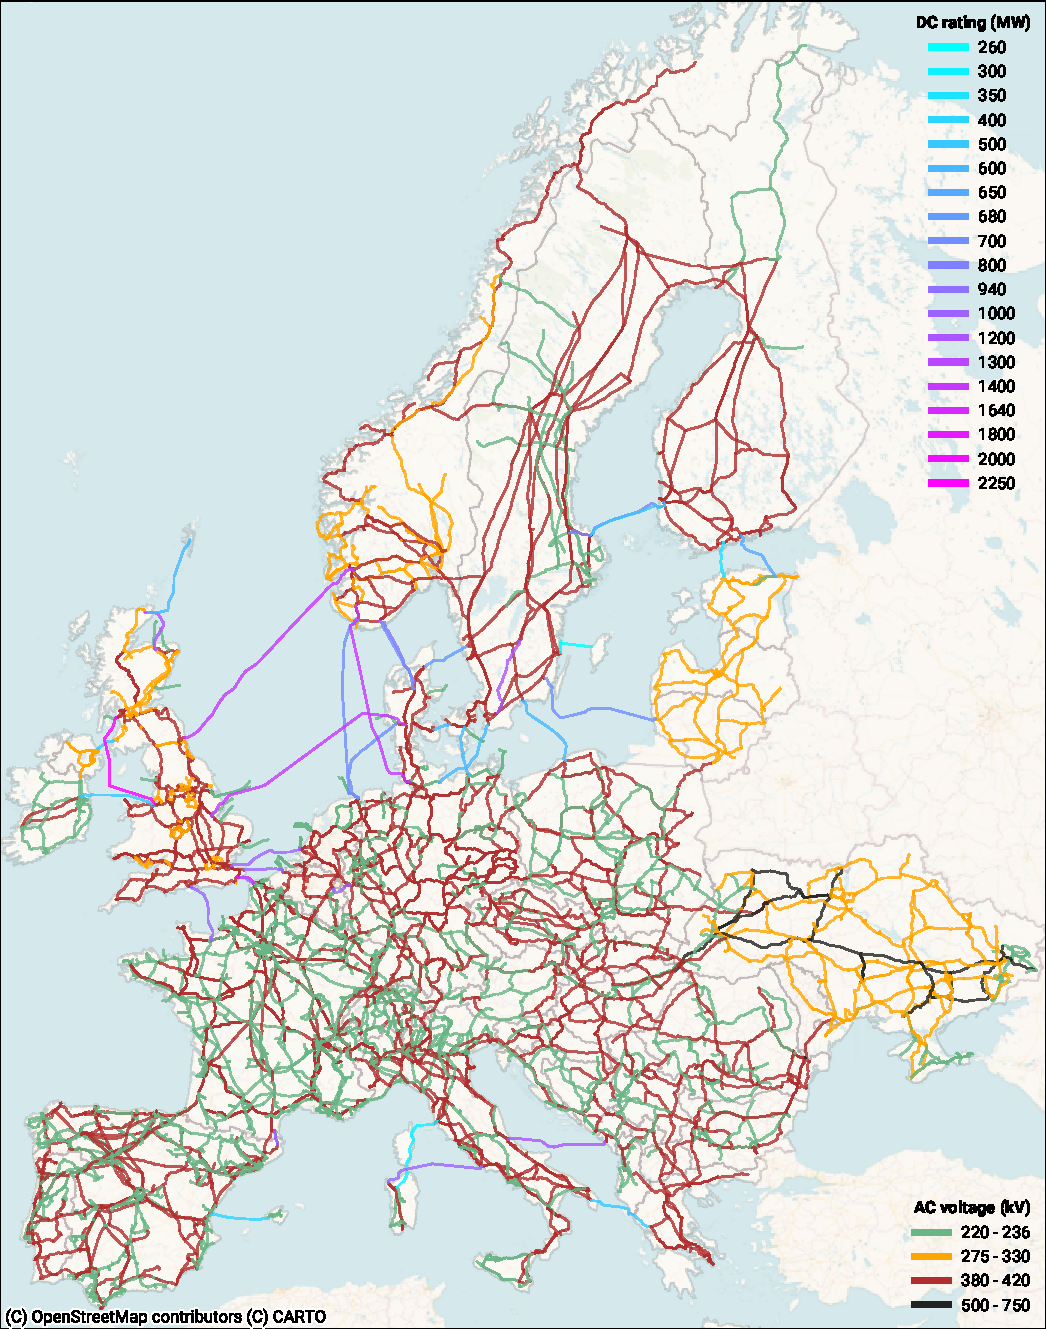
\includegraphics[width=1\textwidth]{osm_map}
		\end{column}
	\end{columns}
	\source{Xiong, Fioriti, Neumann, Riepin, Brown (2025):\\\url{https://www.nature.com/articles/s41597-025-04550-7}; \url{https://github.com/PyPSA/grid-builder}}
\end{frame}

% SLIDE 2: PROLONGED REGIONAL TRANSMISSION OUTAGES
{\setbeamerfont{itemize/enumerate body}{size=\footnotesize}
\begin{frame}{What if Europe's grid breaks into islands for days or weeks?}
	\ongoing
	\vspace{-0.3em}
	\begin{columns}[T,onlytextwidth]
		\begin{column}{0.38\textwidth}
			\centering
			\vspace{0.2em}
			\includegraphics[width=\linewidth,height=0.76\textheight,keepaspectratio]{%
				graphics/resilient-islands/outage_islands_europe.png}\par
			{\tiny\color{mute}Regional islands and transmission line outages (\textcolor{adv}{red})\par}
		\end{column}
		\begin{column}{0.59\textwidth}
			\begin{itemize}\setlength{\itemsep}{0.45em}
				\item \textbf{The threat:} attacks and failures can cut regions off (Baltic cables
				      2023/24, Iberia 2025, Berlin 2025/26), yet planning models assume the grid is
				      always there
				\item \textbf{Our question:} what does it cost for \textbf{every region to ride
					      through on its own} when all links between regions fail for 6\,h to 2~weeks,
				      at the worst time of the year?
				\item \textbf{Europe:} 130 islands of ${\sim}$10\,GW peak load partitioned based on the connectivity of the OSM grid
			\end{itemize}
			\vspace{0.2em}
			\takeaway{\textbf{Relevance:} Outage duration to plan for, minimum reserve requirements (like the EU's 90-day oil stocks), site firm capacity regionally, and
				stress-test grid loss in European/national planning process beyond ERAA.}
		\end{column}
	\end{columns}
	\source{Xiong, Riepin, Brown (2026), working paper}
\end{frame}}

\end{document}
